%-----------------------------------------------------------------------------------------------
\chapter{Algoritmusok, paraméterek}\label{sect:AlgPar}
%-----------------------------------------------------------------------------------------------

A strukturált fényt használó rekonstrukciós eljárások alapja, hogy előre ismert mintát vetítenek a fényképezett objektumra, majd ennek torzulásai alapján következtetnek a mélységinformációra.
A Kinect első verziója is így működik.
Az eszköz mélységképet szolgáltató része (kamera és projektor) az infravörös tartományban üzemel.
A vetített minta egy látszólag véletlenszerű\footnote{Valójában úgy tervezték a pontfelhőt, hogy minimális legyen az egy sorban lévő ismétlődő vagy hasonló blokkok száma} eloszlást követő pontfelhő.
A minta formális leírása vagy a generálás algoritmusa nem ismert, ezért a rekonstrukcióhoz elengedhetetlen valamilyen referenciakép készítése.
A diszparitás meghatározását ez némileg bonyolítja, extra feldolgozási lépéseket tesz szükségessé.

Az extra lépések oka, hogy jelentős időbeli különbség van a referencia- és adatkép készítése között.
Ez idő alatt szinte garantáltan változnak a fényviszonyok, amit kompenzálni kell.
A feladat megoldására 3 lépcsős feldolgozást valósítottam meg, amik a következőkben ismertetésre fognak kerülni.

A rekonstrukció mintaillesztésen alapuló \emph{diszparitás meghatározás}.
Az illeszkedés minőségének javítása érdekében szükség van \emph{előfeldolgozási lépésekre}.
Az diszparitáskép szűrésére és emberi fogyasztásra alkalmassá tételére pedig szükség van \emph{utófeldolgozásra}.

%-----------------------------------------------------------------------------------------------
\section{Előfeldolgozási lépések}\label{sect:Preproc}
%-----------------------------------------------------------------------------------------------

Az előfeldolgozás szükségességét a \figref{needToPreproc} ábra jól mutatja.
Ilyen mértékű fényerőkülönbség esetén a legtöbb mintaillesztési eljárás csődöt mondana.
A jelenség kiküszöbölésére több algoritmust is próbáltam a félév során, melyek változó mértékben voltak eredményesek.
A következőkben ismertetem a kipróbált feldolgozási lépéseket.

\begin{figure}[ht!]
	\begin{subfigure}{.5\textwidth}
	  \centering
	  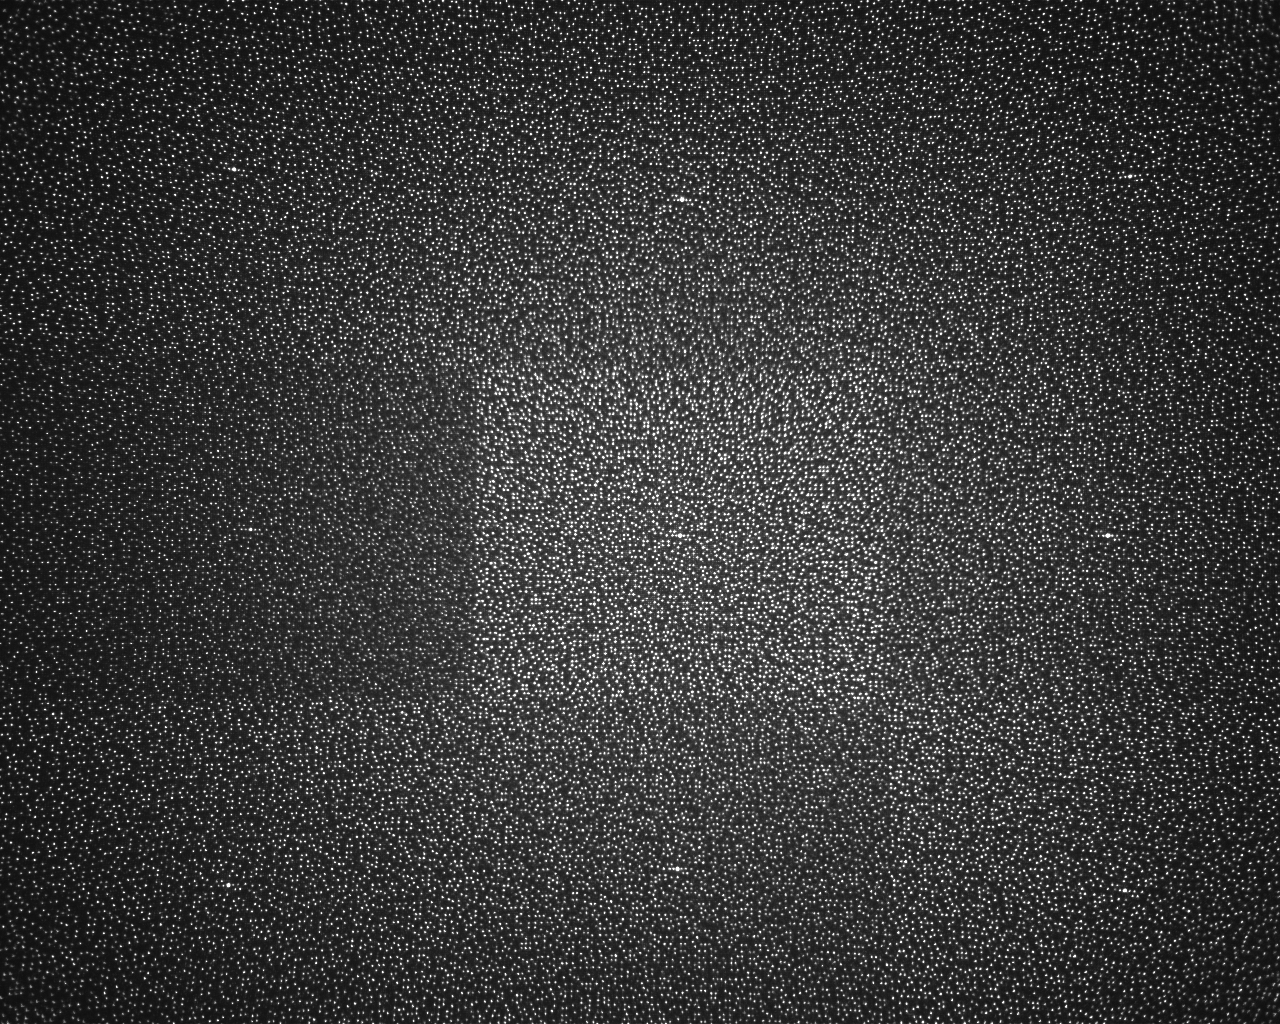
\includegraphics[width=0.9\linewidth]{figures/unproc_ref.png}
	  \caption{Nyers referencia kép}
	  \label{fig:unprocRef}
	\end{subfigure}
	\begin{subfigure}{.5\textwidth}
	  \centering
	  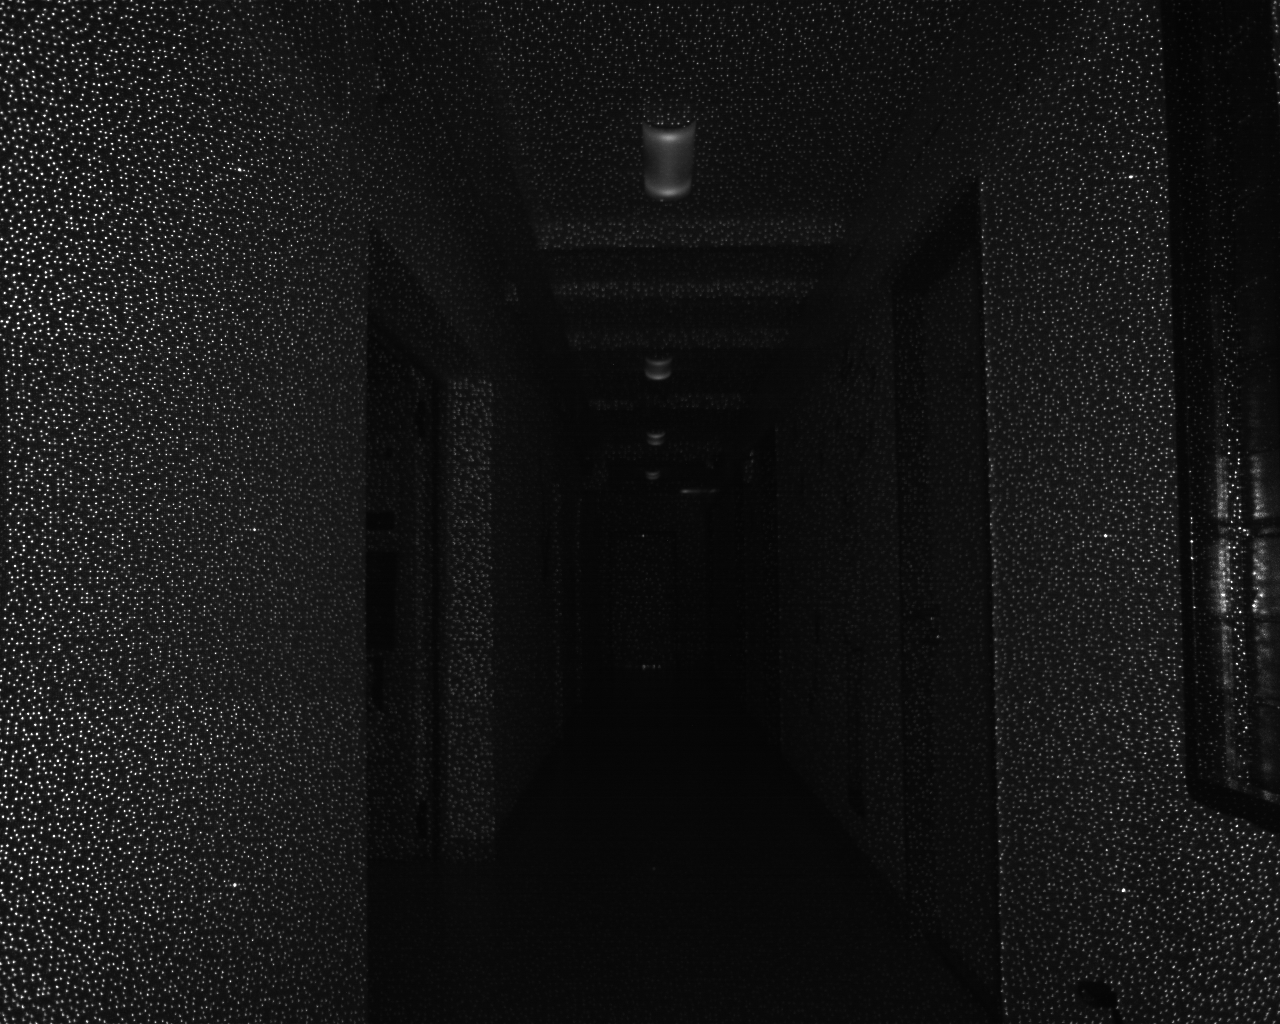
\includegraphics[width=0.9\linewidth]{figures/unproc_data.png}
	  \caption{Nyers adat kép}
	  \label{fig:unprocData}
	\end{subfigure}
	\caption{Fényviszonyok különbsége feldolgozás előtt}
	\label{fig:needToPreproc}
\end{figure}

%-----------------------------------------------------------------------------------------------
\subsection{Difference of Gaussians}\label{sect:DoG}
%-----------------------------------------------------------------------------------------------

Az első ígéretes irány a felüláteresztő szűrés volt.
Ennek egy lehetséges implementáció a DoG algoritmus.
A képet két különböző Gauss szűrővel elmossuk, majd ezeket kivonjuk egymásból.
Gyakran használt szűrő, főleg éldetektálásnál hasznos.
Az én választásom is ezért esett rá: az információ ugyan úgy megtalálható a vetített pontok kontúrjaiban, mint magukban a pontokban.
Képletszerűen \eqref{dog} írja le a műveletet. 

\begin{equation}
dst = gauss(src, \sigma_1) - gauss(src, \sigma_2)
\label{eq:dog}
\end{equation}

A szűrőnek 4 lehetséges paramétere van: a két Gauss szűrő kernel mérete valamint szórása.

%-----------------------------------------------------------------------------------------------
\subsection{Hisztogram kiegyenlítés}\label{sect:histNorm}
%-----------------------------------------------------------------------------------------------

A hisztogram kiegyenlítés ötlete az, hogy a képen belül az összes fényességérték közel azonos mennyiségben legyen reprezentálva.
Erre a műveletre az OpenCV szolgáltat implementált megoldást, aminek használata nagyon praktikus.

A \figref{eqPreproc} ábra mutatja \figref{needToPreproc} képeit hisztogram kiegyenlítés után.
Meg kell jegyezni, hogy az eljárás nem általános megoldás: nem veszi figyelembe a kép lokális tulajdonságait.
A homogén fényerőeloszlás eléréséhez régiónként kellene vizsgálni a képet és egy közös átlagos értékhez igazítani a lokális átlagot.

\begin{figure}[ht!]
	\begin{subfigure}{.5\textwidth}
	  \centering
	  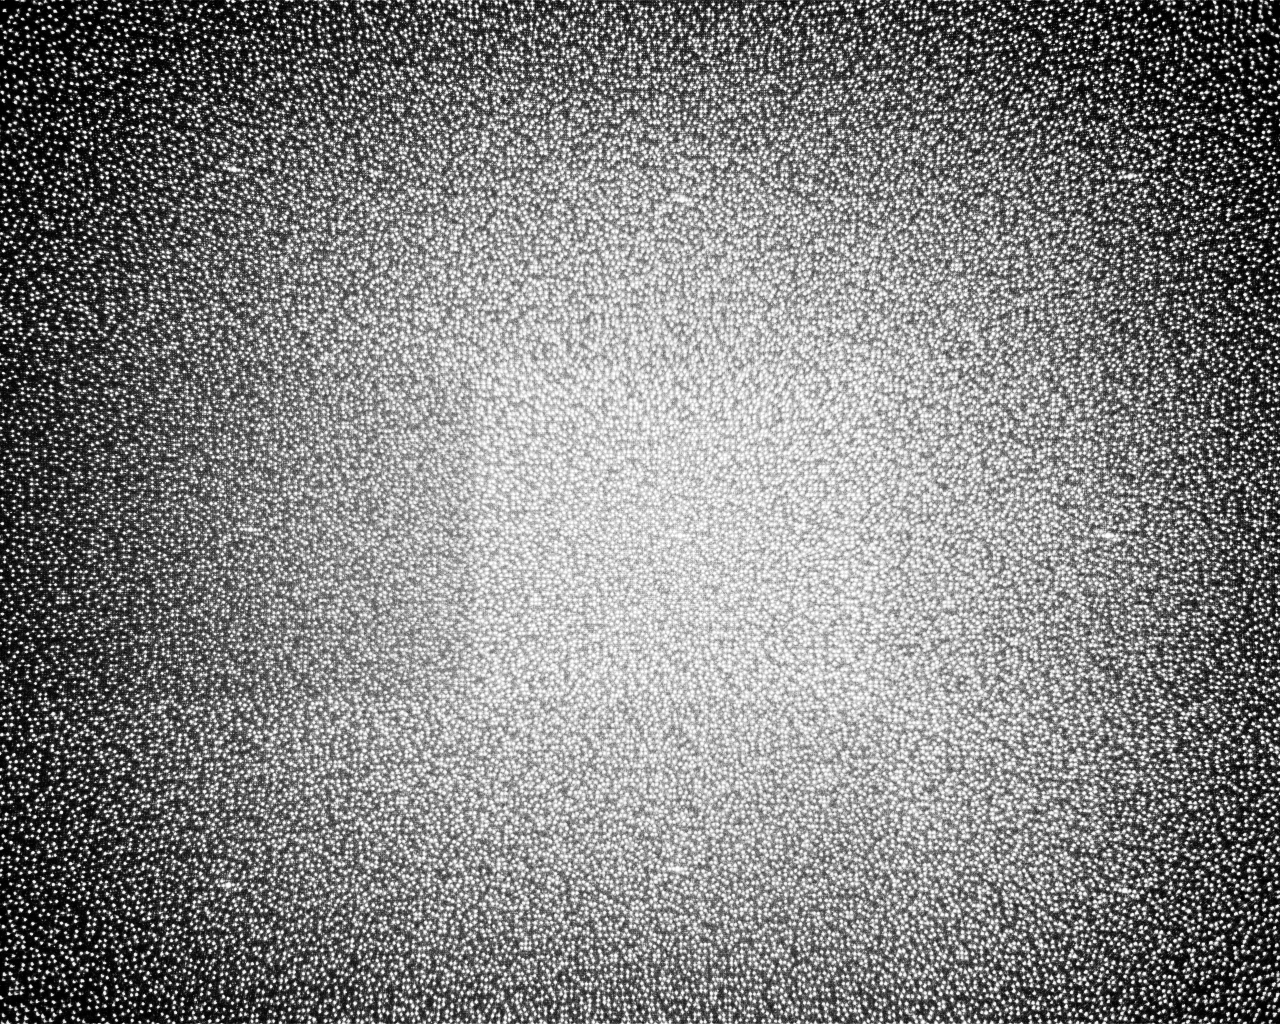
\includegraphics[width=0.9\linewidth]{figures/eq_ref.png}
	  \caption{feldolgozott referencia kép}
	  \label{fig:eqRef}
	\end{subfigure}
	\begin{subfigure}{.5\textwidth}
	  \centering
	  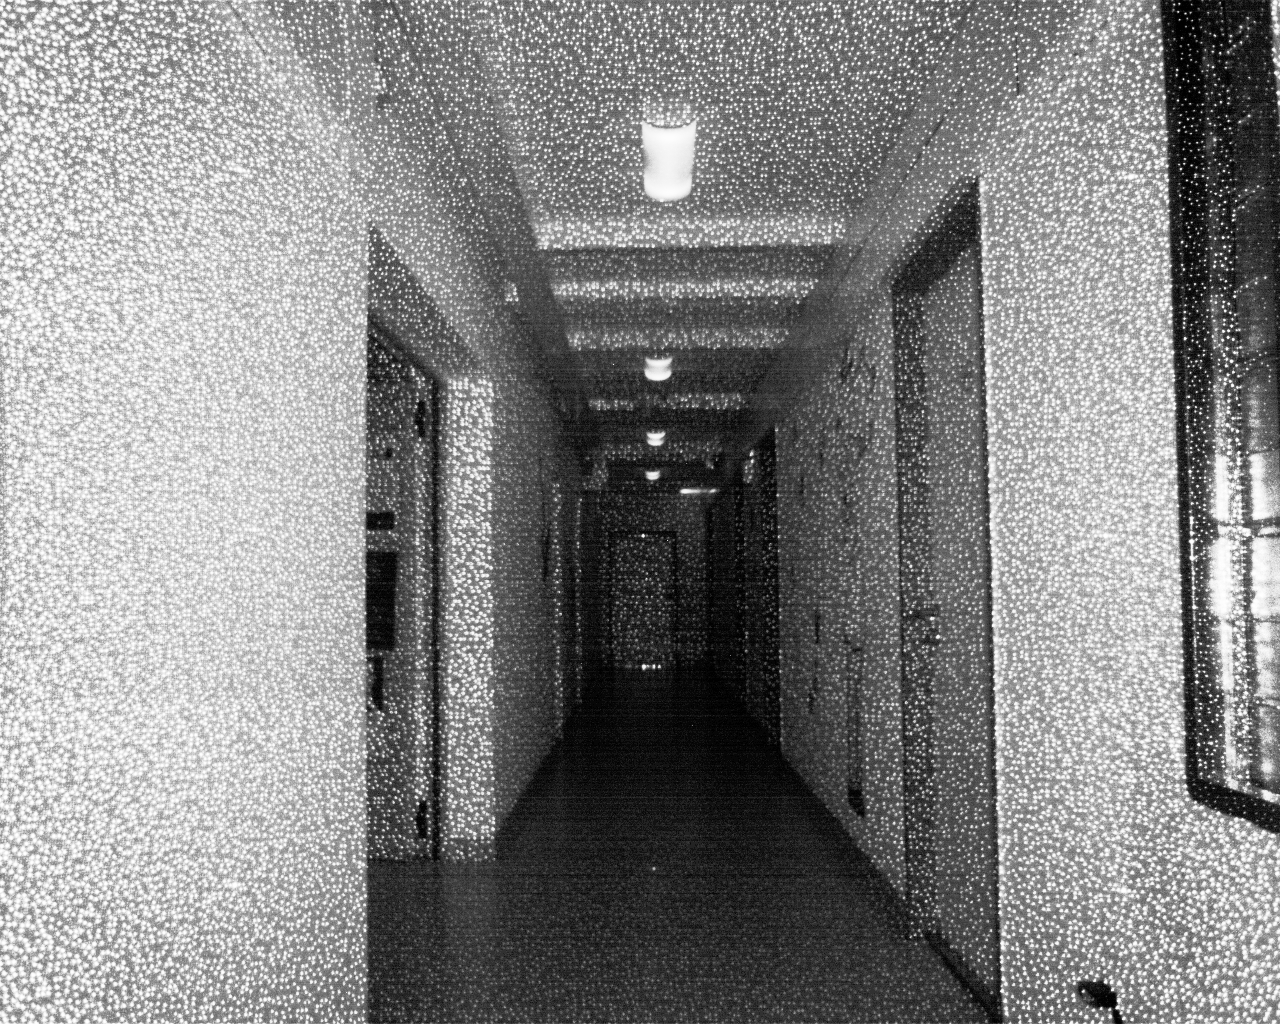
\includegraphics[width=0.9\linewidth]{figures/eq_data.png}
	  \caption{feldolgozott adat kép}
	  \label{fig:eqData}
	\end{subfigure}
	\caption{Hisztogram kiegyenlítés}
	\label{fig:eqPreproc}
\end{figure}

Egy ilyen, lokális tulajdonságokat figyelembe vevő eljárás implementálása szerepel a jövőbeli célok között.
A hisztogram kiegyenlítés használatának egyedüli oka az elfogadható eredmény előállítása és egyszerűsége.

%-----------------------------------------------------------------------------------------------
\subsection{Egyéb előfeldolgozás}\label{sect:miscPreproc}
%-----------------------------------------------------------------------------------------------

Az itt tárgyalt eljárások lényegileg különböznek az eddigiektől.
A fenti algoritmusok a fényességkiegyenlítést szolgálják, míg az alább következők egyéb célokkal kerültek felhasználásra.

%-----------------------------------------------------------------------------------------------
\subsubsection{Uniform skálázás}\label{sect:scale}
%-----------------------------------------------------------------------------------------------

A fejlesztés során két okból került elő ez az egyszerű feldolgozási lépés.
Az első indok a futásidő csökkentése volt.
Gyorsabb volt a kisebb méretű képeken kipróbálni az egyes algoritmus változatokat, mint a teljes elérhető felbontáson.

A másik ok pedig a skálázás diszparitásképre gyakorolt hatásának vizsgálata.
Az volt a megfigyelés, hogy a felére csökkentett méretű képen (640 x 480) simább, kevésbé zajos a kimenet.
Ennek oka az volt, hogy azonos méretű minta nagyobb relatív méretet fedett le a képből, ezért több információt hordozott.
Ehhez adódott még hozzá az a hatás, hogy a felbontás felezése afféle aluláteresztő szűrőként viselkedik.

%-----------------------------------------------------------------------------------------------
\subsubsection{Gauss szűrés}\label{sect:gaussian}
%-----------------------------------------------------------------------------------------------

A Gauss szűrő aluláteresztő jellegű, simítja a képet.
Képfeldolgozási feladatokban gyakran alkalmazzák.
A Gauss kernel elemei egy kétdimenziós normális eloszlás mintái.
Jellemzően 3x3-as vagy 5x5-ös kernelméret a használatos (ez a kép felbontásától erősen függ).

Az két dimenziós eloszlás \eqref{gauss2d} alapján számítható.
\begin{equation}
G_0(x,y) = A e^{\frac{-(x-\mu_x)^2}{2 \sigma_x^2}+\frac{-(y-\mu_y)^2}{2 \sigma_y^2}}
\label{eq:gauss2d}
\end{equation}

A Gauss szűrő paraméterei a kernel méret és az eloszlás szórása.
Általában $\sigma_x$ és $\sigma_y$ megegyezik és négyzetes kernellel dolgozunk, de ettől természetesen el lehet térni.

%-----------------------------------------------------------------------------------------------
\section{Diszparitás meghatározás}\label{sect:Depthproc}
%-----------------------------------------------------------------------------------------------

Az algoritmus futásának ezen szakaszában történik a lényegi 3D információ visszanyerése.
A referenciakép és az adatkép mintái relatív helyzetének a meghatározása a cél.
Ezen probléma megoldására 2 módszer terjedt el: leírók használata vagy mintaillesztés.

A leírókat használó eljárások elemezik a képeket, majd nagy bizonyossággal meghatározható jellegzetes pontokat keresnek.
Ezekből általában kevés van egy képen.
Az ilyen algoritmusok úgynevezett ritka pontfelhős szolgáltatnak kimenetként.

A másik elterjedt út a mintaillesztés használata.
Itt a képek kis régióiból (néhány pixeles környezet) mintát veszünk, és ezeket keressük a másik képen.
Itt az egyezés megbízhatósága jóval kisebb, de cserébe sok adatpontot (sűrű pontfelhő) kapunk.
Ezt a megoldást alkalmaztam a fejlesztés során.

A mintaillesztéses eljárás akkor alkalmazható hatékonyan, ha a képek \emph{rektifikáltak}.
Ez a feltétel a Kinect esetén az eszköz felépítésénél fogva teljesül.

%-----------------------------------------------------------------------------------------------
\subsection{Mintaillesztés}\label{sect:templateMatch}
%-----------------------------------------------------------------------------------------------

A mintaillesztési algoritmus tárgyalásánál a legfontosabb paraméter az illeszkedés jóságát leíró költségfüggvény.
Ezek összehasonlítását és elemzését itt mellőzöm, erről szólt az előző féléves kutatásom.
Itt csak a tapasztalatok által legjobbnak ítélt és azóta használt módszert mutatom be röviden.

A legjobb találati arányt a \emph{normált keresztkorrelációs együtthatót} maximalizáló eljárás adta.
Ennek a számítása költségesebb, mint az általában használt, hibát minimalizáló eljárások (pl. SAD\footnote{Sum of Absolute Differences}).

A költségfüggvény matematika leírása \eqref{NormedCCOEFF} és \eqref{aux_T_I}, ahol $R(x,y)$ jelöli az $(x,y)$ pontra való illeszkedés jóságát.
$T(x,y)$ a referenciakép, $I(x,y)$ pedig az adatkép megfelelő képpontját jelöli.

\begin{equation}\label{eq:NormedCCOEFF}
	\begin{split}
		R(x,y) & = \frac{\sum_{x', y'} (T'(x', y') * I'(x+x', y+y')}{\sqrt{\sum_{x', y'} (T'(x', y')^2 * I'(x+x', y+y')^2)})}
	\end{split}
\end{equation}

\begin{equation}\label{eq:aux_T_I}
	\begin{split}
		T'(x',y') & = T(x',y') - \frac{1}{w*h} * \sum_{x'', y''} T(x'',y'') \\
		I'(x+x',y+y') & = I(x+x',y+y') - \frac{1}{w*h} * \sum_{x'',y''} I(x+x'',y+y'')
	\end{split}
\end{equation}

%-----------------------------------------------------------------------------------------------
\subsection{Paraméterek}\label{sect:params}
%-----------------------------------------------------------------------------------------------

A költségfüggvényen kívül számos egyéb paraméter is befolyásolja a diszparitás sikeres meghatározását.
Ezek inkább az implementációhoz kötődő, a gyakorlatban jelentős jellemzők.

Programozási szemszögből nézve az algoritmus a következőként néz ki.
Mintát kell venni az adatképből, és megkeresni a referenciaképen a legjobban illeszkedő részt.
Ezt a kép minden részére meg kell tenni.
A két képen észlelt pozíciók különbsége a diszparitás.
Annyi könnyebbség adódik, hogy a képek \emph{rektifikáltak}, azaz tudjuk, hogy csak x irányban mozdult el a minta.
Az illeszkedési minőséget minden eltolásra ki kell számolni, ami nagyon számításigényes, lassú művelet.

Optimalizálási céllal nem a teljes tartományon keressük az illeszkedést, hanem feltesszük, hogy egy adott határon belül marad a diszparitás.
Ezt határozza meg az \emph{ablakméret}, amit átlátszó téglalap jelöl a \figref{sizeParams} ábrán.

A másik fontos, méretekkel összefüggő állandó a minta mérete.
Ezt a régiót csúsztatja végig az algoritmus a képen és keresi a referencia képen.
A \figref{sizeParams} ábrán ez a kék négyzettel jelölt tartomány.
Hasonlóan az ablakmérethez, itt is szem előtt kell tartani a teljesítményre gyakorolt hatást.
A kis minta méret rontja az egyedi jelleget, hamis találatokat eredményezhet.
Azonban nem is növelhető tetszőlegesen, mert akkor már túl nagy lesz az eltérés a referencia és az adat között (itt a kép tartalma okozza a hibát).

Az ablak méretnek legalább el kell érnie a minta méretét.

\begin{figure}[ht!]
	\centering
	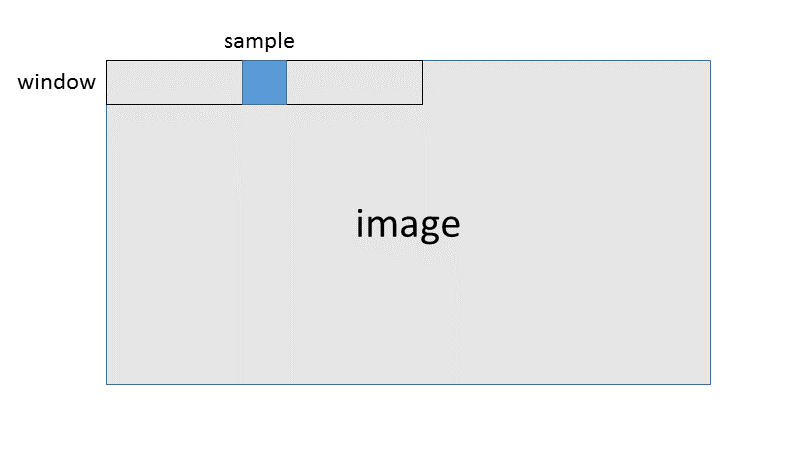
\includegraphics[width=0.7\linewidth]{figures/sizeParams.png}
	\caption{Méret paraméterek}
	\label{fig:sizeParams}
\end{figure}

Fontos megjegyezni, hogy ezek azok a paraméterek, amik az összes feldolgozási stratégiára jellemzők függetlenül attól, hogy figyelembe vesszük-e a lokális képi struktúrát.

%-----------------------------------------------------------------------------------------------
\section{Utófeldolgozás}\label{sect:Postproc}
%-----------------------------------------------------------------------------------------------

Az utófeldolgozási fázisban az előállított diszparitáskép manipulációja történik.
Alkalmazhatóak zajszűrő eljárások, de akár lehet szó egyszerű vizualizációról is.
Érdemi 3D feldolgozás nem történik itt, csak az eredmény kisebb-nagyobb formázása.

A munka nagy részében kizárólag vizualizáció történt ebben a fázisba.
Folytattam kísérleteket medián szűrő alkalmazásával is.
Ennek (jelen féléves projekt keretei között) nincs gyakorlati jelentősége: még a diszparitás számítási fázisban próbáltam a zajszűrést elvégezni.

%-----------------------------------------------------------------------------------------------
\subsection{Medián szűrő}\label{sect:median}
%-----------------------------------------------------------------------------------------------

A medián szűrő nem lineáris szűrő.
Az úgynevezett rang szűrők közé tartozik.
Működési elve: a kernelben található képpontokat érték szerint sorba rendezi, majd a kernelközéppont értékét helyettesíti az elemek mediánjával.
Kiválóan alkalmas pontszerű hibák szűrésére.

A fent említett tulajdonsága miatt merült fel a használata.
A kezdeti próbálkozások kimeneti képei ilyen jellegű hibával terheltnek látszottak.
Mint további vizsgálat alapján kiderült, a hibák nem pontszerűek, túl nagy a kiterjedésük ahhoz, hogy ésszerű kernelméretű mediánszűrő kezelni tudja őket.
Ilyen jellegű zajjal terhelt képet mutat a \figref{medianReason} ábra.

\begin{figure}[ht!]
	\centering
	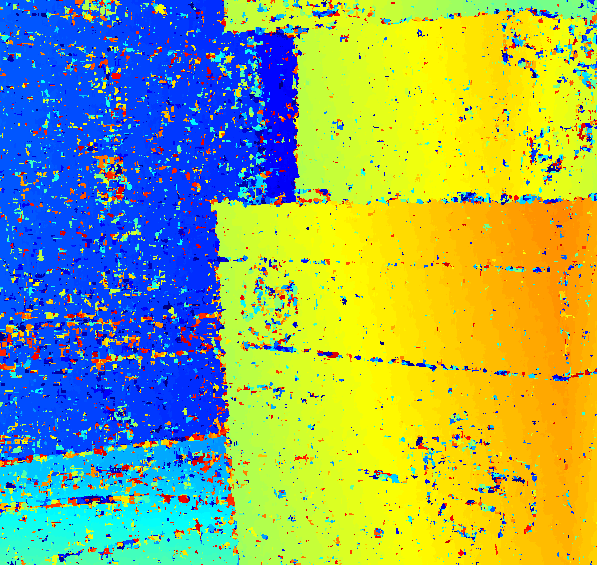
\includegraphics[width=0.6\linewidth]{figures/medianreason.png}
	\caption{Zajjal terhelt kimeneti kép}
	\label{fig:medianReason}
\end{figure}

%-----------------------------------------------------------------------------------------------
\subsection{Vizualizáció}\label{sect:visual}
%-----------------------------------------------------------------------------------------------

Ez a lépés arra szolgál, hogy könnyen átlátható formában jelenítse meg a diszparitást.
Nyers formájukban a kapott értékek igen alacsonyak és monokromatikusak.
Ez egy alacsony átlagos intenzitású, szürkeárnyalatos képet eredményez.
Ez a feldolgozási szakasz interpolálja a kapott számértékeket RGB képre.
A képen a közeli pontok vörössel, a távoliak kékkel vannak jelölve, köztük pedig folytonosan változik a szín a diszparitás nagyságával arányosan.
Fontos megjegyezni, hogy ez \emph{nem mélységkép}, csak a diszparitás megjelenítése.
Ezen eljárás kimenete a \figref{medianReason} ábra is.
